\documentclass[tikz,border=8pt]{standalone}
\usetikzlibrary{arrows.meta,backgrounds,fit,positioning}

\definecolor{deployblue}{HTML}{D9EAF7}
\definecolor{deploygreen}{HTML}{D9EAD3}
\definecolor{deployyellow}{HTML}{FFF2CC}
\definecolor{deploygray}{HTML}{F2F2F2}
\definecolor{deployline}{HTML}{4F6D7A}

\tikzset{
  service/.style={
    draw=deployline,
    rounded corners=2pt,
    fill=#1,
    minimum width=3.0cm,
    minimum height=1.05cm,
    align=center,
    font=\sffamily\small
  },
  service/.default=deploygray,
  store/.style={
    draw=deployline,
    rounded corners=2pt,
    fill=deployyellow,
    minimum width=2.75cm,
    minimum height=0.95cm,
    align=center,
    font=\sffamily\small
  },
  arrow/.style={-Latex,thick,draw=deployline},
  group/.style={draw=deployline,rounded corners=4pt,dashed,inner sep=8pt}
}

\begin{document}
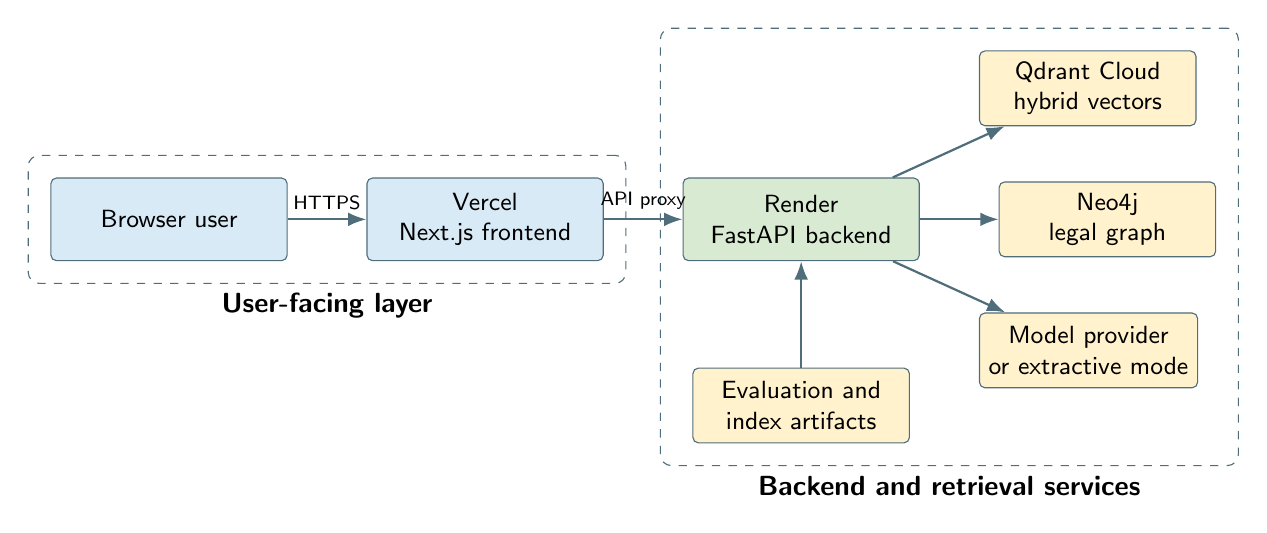
\begin{tikzpicture}[node distance=0.9cm and 1.0cm]
  \node[service=deployblue] (browser) {Browser user};
  \node[service=deployblue, right=of browser] (vercel) {Vercel\\Next.js frontend};
  \node[service=deploygreen, right=of vercel] (render) {Render\\FastAPI backend};

  \node[store, above right=0.65cm and 0.75cm of render] (qdrant) {Qdrant Cloud\\hybrid vectors};
  \node[store, right=of render] (neo4j) {Neo4j\\legal graph};
  \node[store, below right=0.65cm and 0.75cm of render] (provider) {Model provider\\or extractive mode};
  \node[store, below=1.35cm of render] (artifacts) {Evaluation and\\index artifacts};

  \draw[arrow] (browser) -- node[above,font=\sffamily\scriptsize]{HTTPS} (vercel);
  \draw[arrow] (vercel) -- node[above,font=\sffamily\scriptsize]{API proxy} (render);
  \draw[arrow] (render) -- (qdrant);
  \draw[arrow] (render) -- (neo4j);
  \draw[arrow] (render) -- (provider);
  \draw[arrow] (artifacts) -- (render);

  \begin{scope}[on background layer]
    \node[group,fit=(browser)(vercel),label={[font=\sffamily\bfseries]below:User-facing layer}] {};
    \node[group,fit=(render)(qdrant)(neo4j)(provider)(artifacts),label={[font=\sffamily\bfseries]below:Backend and retrieval services}] {};
  \end{scope}
\end{tikzpicture}
\end{document}
